\documentclass{article}

\usepackage[english]{babel}

\usepackage[a4paper,top=2cm,bottom=2cm,left=3cm,right=3cm,marginparwidth=1.75cm]{geometry}

% Useful packages
\usepackage{amsmath}
\usepackage{graphicx}
\usepackage[colorlinks=true, allcolors=blue]{hyperref}
\usepackage{multicol}
\usepackage{subcaption}
\usepackage{siunitx}
\usepackage{afterpage}

\usepackage{tikz}
\usetikzlibrary{shapes.geometric, arrows}
\tikzstyle{startstop} = [rectangle, rounded corners, minimum width=3cm, minimum height=1cm,text centered, draw=black, fill=red!30]
\tikzstyle{pimage} = [rectangle, minimum width=3cm, minimum height=1cm, text centered, draw=black, fill=orange!30]
\tikzstyle{pline} = [rectangle, minimum width=3cm, minimum height=1cm, text centered, draw=black, fill=blue!30]
\tikzstyle{pfft} = [rectangle, minimum width=3cm, minimum height=1cm, text centered, draw=black, fill=green!30]
\tikzstyle{arrow} = [thick,->,>=stealth]

\newcommand\todo[1]{\textcolor{red}{\bf TODO: #1}}

\title{Detecting Moving Objects in DAS Recordings}
\author{
  Patryk Janiak\\
  \texttt{156053}
  \and
  Marek Seget\\
  \texttt{156042}
}

\begin{document}
\maketitle

\begin{abstract}
Develop an algorithm to detect and track moving objects in acoustic data collected from a Distributed Acoustic Sensing (DAS) system.
\end{abstract}

\section{Introduction}
Distributed Acoustic Sensing (DAS) is an advanced technology that transforms optical fiber cables into highly sensitive vibration sensors. By sending pulses of laser light through a fiber optic cable and analyzing the backscattered light, DAS systems can detect subtle strain variations along the fiber, which may be caused by seismic activity, traffic, or small object movements. These variations are recorded as phase shifts in the backscattered light signal, which correlate directly to the fiber's strain. With appropriate calibration, these phase shifts are processed to measure strain or strain rate over time. The resulting time-series data provides a detailed, chronological record of vibrations along the fiber, allowing for further analysis to identify the source, magnitude, and frequency of disturbances.

\section{Data set}
The data is stored in numpy format as a 2D matrix. The particular value represents the strain rate of a fiber optic cable located on a busy street (Jana Pawla II). The data shows the passage of trams, trucks or cars along this street.
The first dimension is time, the second is space, in order to calculate the correct units use the following metadata:

\begin{multicols}{2}
\begin{itemize}
\item dx: 5.106500953873407 [m]
\item dt: 0.0016 [s]
\item file duration: 10s
\item number of time samples in file: 6250
\item file name format: HHMMSS
\item files date: 2024-05-07
\end{itemize}
\end{multicols}

\subsection{Analysis}

Input values range from \numrange{-4.4314038e-05}{4.4261396e-05}. The mean is \num{4.4261396e-05} and the median is \num{0}. The distribution is normal as seen in Figure 1.

\begin{figure}[htbp]
    \centering
    \includegraphics[width=0.45\linewidth]{da1.2.png}
    \caption{Histogram of input values clipped from \numrange{-1e-6}{1e-6}.}
    \label{fig:da12}
\end{figure}

\newpage
\section{Algorithm}

% \centering
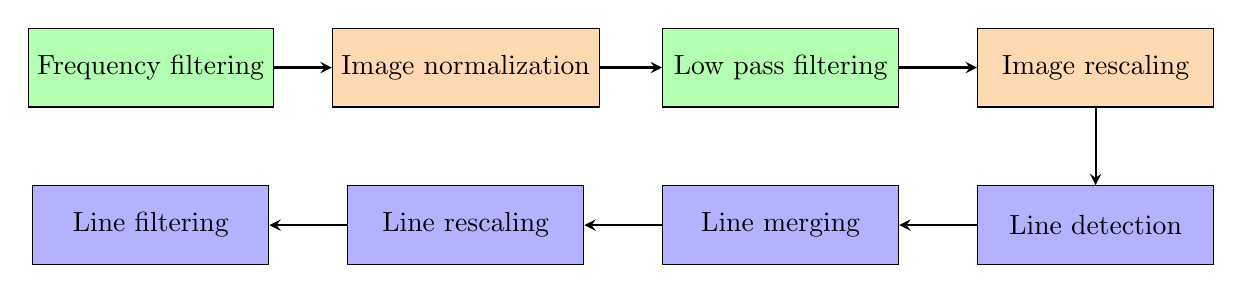
\begin{tikzpicture}[node distance=2cm]
\node (freq) [pfft] {Frequency filtering};
\node (norm) [pimage, right of=freq, xshift=2cm] {Image normalization};
\node (noise) [pfft, right of=norm, xshift=2cm] {Low pass filtering};
\node (rescale) [pimage, right of=noise, xshift=2cm] {Image rescaling};
\node (detect) [pline, below of=rescale] {Line detection};
\node (merge) [pline, left of=detect, xshift=-2cm] {Line merging};
\node (lrescale) [pline, left of=merge, xshift=-2cm] {Line rescaling};
\node (lfilter) [pline, left of=lrescale, xshift=-2cm] {Line filtering};
\draw [arrow] (freq) -- (norm);
\draw [arrow] (norm) -- (noise);
\draw [arrow] (noise) -- (rescale);
\draw [arrow] (rescale) -- (detect);
\draw [arrow] (detect) -- (merge);
\draw [arrow] (merge) -- (lrescale);
\draw [arrow] (lrescale) -- (lfilter);
\end{tikzpicture}

\subsection{Frequency filtering}
Using Discrete Fourier Transform sample frequencies we can filter out frequencies lesser than 40Hz and bigger than 60Hz. These frequencies were optimally chosen by trial and error.

\subsection{Image normalization}
Normalize the values into a range from \numrange{0}{255}. First, shift the mean to zero and take the absolute value. Then, clip the values below 99th percentile. Finally, scale it to be between 0 and 255.

\subsection{Low pass filtering}
Next, we perform low pass filtering in the frequency domain. This helps remove the noise from the background and smooth out the remaining lines.

\subsection{Image rescaling}
The original data has the shape 75000 by 52. Because of the extreme aspect ratio, we opted to downscale the image's height to 256. We also decided to upscale the image's width to 256 as this proved to help with the next step.

\subsection{Line detection}
In order to detect lines we used the probabilistic hough lines with threshold equal to 100, minimum line length equal to 4 and maximum line gap equal to 128. We optimized the parameters by trial and error.

\subsection{Line merging}
We calculate the average distance between each pair of lines using an integral that measures the absolute difference between their linear functions over their overlapping intervals.

\[
\bar{d} = \frac{\int_{a}^{b} |f(x) - g(x)| \,dx}{b - a}, b > a
\]

\noindent This results in a distance matrix where each entry reflects the average distance between two lines.

Next, the algorithm applies the DBSCAN clustering method to this distance matrix, allowing it to automatically determine clusters based on the density of lines in the feature space.

After clustering, the algorithm merges lines within each cluster by averaging their endpoint coordinates, creating new line segments that represent the collective geometry of the clustered lines.

\subsection{Line rescaling}
Due to the lines being produced on a decimated image we need to rescale them back to the original image size. Now we can calculate $speed = \frac{1}{|a|}*\frac{dx}{dt}*3.6$ in km/h.
% $speed = |\frac{dx * 3600}{a * dt * 1000}|$

\subsection{Line filtering}
Also, we know that there shouldn't be any vertical lines (indicating no movement) and horizontal lines (indicating instantaneous movement). Thus we limited the angle of the lines to be between 1km/h and 200km/h.

\afterpage{\clearpage}
\begin{figure}[p]
    \centering
    \begin{subfigure}{0.45\textwidth}
        \centering
        \includegraphics[width=\linewidth]{filtered_and_normalised.png}
        \caption{Filtered frequencies and normalized data}
        \label{fig:freqnorm}
    \end{subfigure}
    \hfill
    \begin{subfigure}{0.45\textwidth}
        \centering
        \includegraphics[width=\linewidth]{low_filtered.png}
        \caption{Low pass filtering}
        \label{fig:lowfilt}
    \end{subfigure}

    \begin{subfigure}{0.45\textwidth}
        \centering
        \includegraphics[width=\linewidth]{downsampled.png}
        \caption{Resized image}
        \label{fig:down}
    \end{subfigure}
    \hfill
    \begin{subfigure}{0.45\textwidth}
        \centering
        \includegraphics[width=\linewidth]{hough.png}
        \caption{Probabilistic hough lines}
        \label{fig:houg}
    \end{subfigure}

    \begin{subfigure}{0.45\textwidth}
        % \centering
        \includegraphics[width=\linewidth]{clustered.png}
        \caption{Clustered based on $\bar{d}$}
        \label{fig:cluster}
    \end{subfigure}
    \hfill
    \begin{subfigure}{0.45\textwidth}
        \centering
        \includegraphics[width=\linewidth]{merged.png}
        \caption{Merged lines}
        \label{fig:merged}
    \end{subfigure}
\end{figure}

\newpage
\section{Results}

\begin{figure}[htbp]
    \centering
    \begin{subfigure}{0.45\textwidth}
        \centering
        \includegraphics[width=\linewidth]{janiak_range.png}
        \caption{Janiak's range [091052, 091242]}
        \label{fig:sub1}
    \end{subfigure}
    \hfill
    \begin{subfigure}{0.45\textwidth}
        \centering
        \includegraphics[width=\linewidth]{seget_range.png}
        \caption{Seget's range [090252, 090442]}
        \label{fig:sub2}
    \end{subfigure}

    \begin{subfigure}{0.45\textwidth}
        \centering
        \includegraphics[width=\linewidth]{unassigned_range.png}
        \caption{Unassigned range [093652, 093842]}
        \label{fig:sub3}
    \end{subfigure}

\end{figure}

The algorithm has no issues with detecting thick and medium lines but has some troubles with highlighting short and faint lines. Thanks to noise filtering, even in the very noisy 3rd range most lines are correctly labeled.

\newpage
\section{Other approaches}
\todo{Show all the failed experiments as subfigures}

\section{Conclusion}
The described algorithm proved to provide the best results. \todo{reiterate the algorithm}

% \bibliographystyle{alpha}
% \bibliography{sample}

\end{document}
